\documentclass{article}

% if you need to pass options to natbib, use, e.g.:
%     \PassOptionsToPackage{numbers, compress}{natbib}
% before loading neurips_2024

% ready for submission
\usepackage[final]{neurips_2024}

\usepackage[utf8]{inputenc} % allow utf-8 input
\usepackage[T1]{fontenc}    % use 8-bit T1 fonts
\usepackage{hyperref}       % hyperlinks
\usepackage{url}            % simple URL typesetting
\usepackage{booktabs}       % professional-quality tables
\usepackage{amsfonts}       % blackboard math symbols
\usepackage{nicefrac}       % compact symbols for 1/2, etc.
\usepackage{microtype}      % microtypography
\usepackage{xcolor}         % colors
\usepackage{graphicx}
\usepackage{amssymb,amsmath}
\usepackage{subcaption}
\usepackage{makecell}
\usepackage{float}

% APA author-year citations (required by Neural Networks journal)
\usepackage{natbib}

\title{Modular vs.\ Monolithic Neural Networks in a Causal Chain (DRAFT)}
\author{%
  Safaa Hassan \\
  \texttt{safaahassan@college.harvard.edu} 
  \And
  Sarra Guezguez \\
  \texttt{sarra\_guezguez@college.harvard.edu} 
  \And
  Linbo Tang \\
  \texttt{linbotang@g.harvard.edu} 
}


\begin{document}

\maketitle

% 
% KEYWORDS (required by Neural Networks / Elsevier; enter these
% in the online submission system — 1 to 6 keywords)
% modular neural networks, causal inference, distribution shift,
% few-shot adaptation, compositional generalization, causal mechanisms
% 

\begin{abstract}
Modular neural architectures, whose sub-networks mirror individual causal
mechanisms, offer a parameter-efficient pathway for adapting to localized changes
in a data-generating process, but their advantage over monolithic models has not
been cleanly isolated in a controlled causal setting.
We address this gap by training and evaluating both architecture types on synthetic
data drawn from causal chains of depth three ($A\!\rightarrow\!B\!\rightarrow\!C$)
and four ($A\!\rightarrow\!B\!\rightarrow\!C\!\rightarrow\!D$) nodes, then
intervening on a single upstream mechanism at test time.
In-distribution, both architectures achieve comparable mean squared error.
Under the intervention, neither achieves zero-shot robustness regardless of
architectural decomposition, but modular models adapt substantially more
efficiently in the few-shot regime: with only 50 interventional samples, the
modular model reduces MSE by 24\% relative to the monolithic baseline, an advantage
that diminishes as sample size grows.
In the deeper four-node chain, modular models also attain lower final error after
adaptation despite updating only the perturbed module.
These results provide controlled empirical evidence that aligning model structure
with the causal factorization of the environment improves adaptation efficiency,
especially in low-data regimes and deeper compositional settings, while highlighting
that architectural modularity alone is insufficient for zero-shot robustness under
severe mechanism shifts.
\end{abstract}

\noindent\textbf{Keywords:} modular neural networks; causal mechanisms; distribution shift; few-shot adaptation; compositional generalization; causal chains


\section{Introduction}
\label{sec:intro}

Modular neural networks can adapt to a localized causal change by retraining only
the module aligned with the altered mechanism, while leaving unaffected modules
frozen. Whether this structural advantage translates into measurable gains over a
monolithic baseline - and under what conditions - has not been tested in a clean
causal setting. We address that question directly.

Many real-world systems are governed by multiple processes that operate
independently and compose to produce observable outcomes. When such systems undergo
change, typically only a subset of the underlying mechanisms is modified while the
others remain stable \citep{pearl2009causality}. Standard neural networks tend to
learn entangled representations \citep{locatello2019challenging} that do not reflect
this structure; as a result, a monolithic model trained end-to-end may perform well
in-distribution yet fail when the distribution shifts due to a change in one causal
mechanism. Architectures that mirror the factorization of the generative process may
possess a more appropriate inductive bias for handling such interventions
\citep{bengio2019meta}.

We test this idea in a controlled synthetic environment defined by the causal chain
$A\!\rightarrow\!B\!\rightarrow\!C$, where two independent nonlinear mechanisms
allow us to intervene on one while holding the other fixed. We extend the setting
to a four-node chain $A\!\rightarrow\!B\!\rightarrow\!C\!\rightarrow\!D$ to examine
whether the depth of the causal composition amplifies any modular effect. The
modular model consists of sub-networks trained with local supervision on each
mechanism; the monolithic baseline is a standard MLP trained end-to-end. After
intervening on the upstream mechanism at test time, we evaluate both zero-shot
generalization and few-shot adaptation across a range of sample sizes.

Our main findings are: (1) both architectures match in-distribution; (2) neither
achieves zero-shot robustness under a severe functional shift; (3) modular models
adapt more parameter-efficiently, with the largest relative gains (24\%) at the
smallest sample sizes; and (4) the modular advantage in final adapted accuracy
grows with causal depth. These results suggest that explicit compositional
structure serves as a useful inductive bias for adaptation under localized causal
change, while underscoring that modularity alone does not confer zero-shot
robustness.


\section{Related Work}
\label{sec:related}

\subsection{Causal models and independent mechanisms}

Structural causal models formalize how interventions modify specific mechanisms
while leaving others invariant \citep{pearl2009causality}, and this autonomy
property underpins approaches that exploit invariant structure across environments.
Invariant prediction methods identify causal relations by seeking components that
remain stable across distributional shifts \citep{peters2016causal}, while causal
representation learning emphasizes encoding mechanisms that are robust to
interventions \citep{scholkopf2021toward}. Recent work has extended these ideas to
large-scale neural systems: \citet{gendron_icm_llms} report improved
out-of-distribution reasoning when architectures reflect the Independent Causal
Mechanisms principle, and \citet{pruthi_compositional_causal} show that decomposing
causal components improves generalization when underlying mechanisms vary across
units.

\subsection{Modular neural architectures}
Neural Module Networks demonstrated how task-specific computations can be composed
from learned modules \citep{andreas2016neural}. Subsequent work proposed
self-organizing modular networks \citep{jiang2019self}, routing networks that
adaptively select among subcomponents \citep{rosenbaum2017routing}, and Recurrent
Independent Mechanisms \citep{goyal2019recurrent}.
\citet{schug_modular_solutions} show that module-wise factorization improves
generalization to unseen compositions, and \citet{locatelli_modularity} find that
modular networks support systematic generalization by reusing functional components.
In contrast to these works, which focus on compositional generalization, our
emphasis is on whether alignment with a known causal decomposition yields advantages
specifically under targeted interventions.

\subsection{Symbolic and neurosymbolic perspectives}
Classical expert systems \citep{shortliffe1976mycin,lindsay1980dendral} and
cognitive theories including Minsky's Society of Mind \citep{minsky_society_of_mind}
and Bayesian Program Learning \citep{lake_program_induction} illustrate how
compositional structure can support selective updating. Neurosymbolic
approaches-including the Neuro-Symbolic Concept Learner \citep{mao_nsc} and
Rational Meaning Construction \citep{wong_rmc}-further reinforce this potential.
Our contribution is complementary to this, testing whether purely neural modular
architectures inherit the selective-update advantage in a tightly controlled causal
setting.


\section{Methods}
\label{sec:method}

\subsection{Environment and Causal Structure}

We study both architectures in a controlled environment defined by the causal chain
$A \rightarrow B \rightarrow C$, where $A \in \mathbb{R}^4$, $B \in \mathbb{R}^3$,
and $C \in \mathbb{R}^3$. Figure~\ref{fig:causal_diagram} illustrates the
data-generating process. Each arrow represents a distinct, independent causal
mechanism.

The upstream mechanism $A \rightarrow B$ uses nonlinear combinations of components
of $A$: $\sin(A_1)$, $A_2^2$, $A_3 \cdot \sigma(A_4)$, and $e^{-|A_2|}$.
The downstream mechanism $B \rightarrow C$ applies fixed nonlinear transformations
including $\tanh(w_1^\top B)$, $\mathrm{ReLU}(w_2^\top B)$, multiplicative
interactions, and $\cos(B_3)$. These mechanisms satisfy the assumption of
independent causal mechanisms, enabling us to modify one while holding the other
fixed.

\begin{figure}[H]
    \centering
    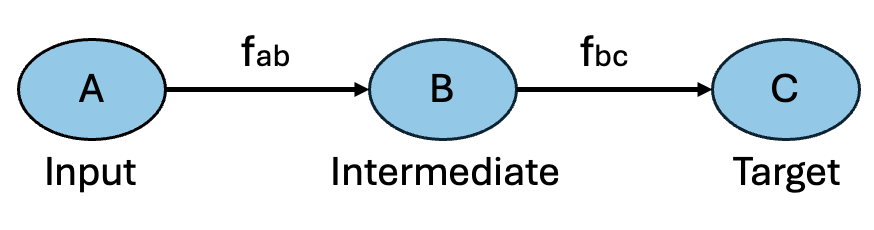
\includegraphics[width=0.6\linewidth]{causal_diagram.png}
    \caption{Causal chain: the observational environment consists of two independent
    mechanisms $A \rightarrow B$ and $B \rightarrow C$.}
    \label{fig:causal_diagram}
\end{figure}

We compare two architectures:
\begin{itemize}
    \item \textbf{Monolithic model} (Figure~\ref{fig:monolithic_model}): a single
    MLP trained end-to-end to map $A \mapsto C$, with no access to or supervision
    on $B$.
    \item \textbf{Modular model} (Figure~\ref{fig:modular_model}): two sub-networks,
    $f_{AB}: A \mapsto B$ and $f_{BC}: B \mapsto C$, each supervised with a local
    loss corresponding to its target variable.
\end{itemize}

\begin{figure}[H]
    \centering
    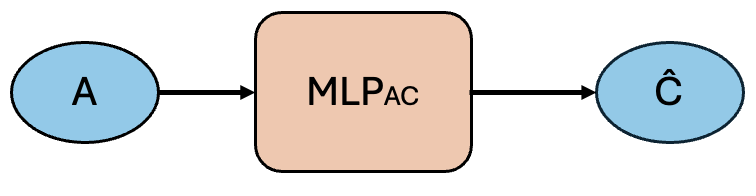
\includegraphics[width=0.4\linewidth]{monolithic_model.png}
    \caption{Monolithic architecture: a single network learns the composite mapping
    $A \mapsto C$ without intermediate supervision.}
    \label{fig:monolithic_model}
\end{figure}

\begin{figure}[H]
    \centering
    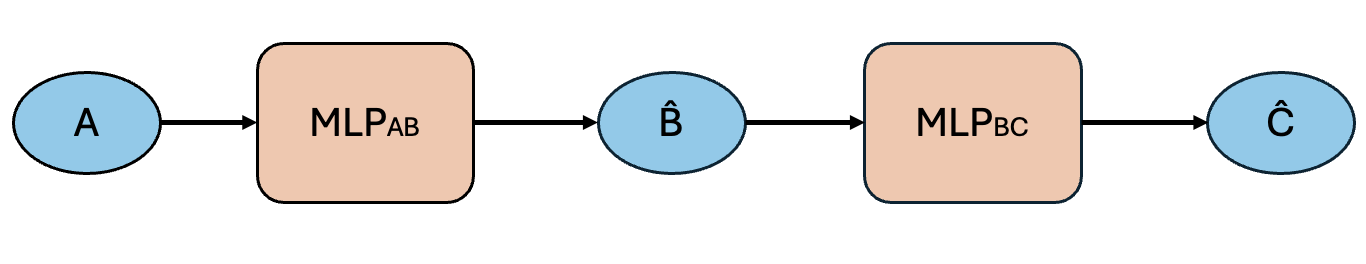
\includegraphics[width=0.7\linewidth]{modular_model.png}
    \caption{Modular architecture: two sub-networks separately learn $f_{AB}$ and
    $f_{BC}$, mirroring the causal structure of the generative process.}
    \label{fig:modular_model}
\end{figure}

Both models are trained on 20{,}000 observational samples and evaluated on a
held-out test set of 5{,}000 samples.

\subsection{Intervention Design}

We intervene \emph{only} on the upstream mechanism $A \rightarrow B$.
The observational mechanism is:
\[
\begin{aligned}
B_1 &= \sin(A_1) + 0.5\,A_2^2 + \epsilon_1, \\
B_2 &= A_3 \cdot \sigma(A_4) + \epsilon_2, \\
B_3 &= e^{-|A_2|} + 0.1A_1 + \epsilon_3,
\end{aligned}
\]
where $\sigma(\cdot)$ is the logistic sigmoid and
$\epsilon_i \sim \mathcal{N}(0, \sigma^2)$.

The intervened mechanism replaces each component:
\[
\begin{aligned}
B_1' &= \cos(A_1) + 0.5\,A_2^3 + \epsilon_1', \\
B_2' &= - A_3 \cdot \sigma(A_4) + \epsilon_2', \\
B_3' &= e^{-|A_2|} - 0.2A_1 + \epsilon_3'.
\end{aligned}
\]

This introduces three independent shifts: a phase and nonlinearity change
($\sin \rightarrow \cos$, quadratic $\rightarrow$ cubic), a sign inversion in the
interaction term, and a change in the linear dependence of $B_3$ on $A_1$.
The downstream mechanism $B \rightarrow C$ is held fixed throughout, ensuring that
performance degradation is attributable solely to the upstream intervention.

\subsection{Evaluation Protocol}

We evaluate each model under three conditions:
\begin{enumerate}
    \item \textbf{In-distribution:} MSE on the observational environment.
    \item \textbf{Zero-shot:} MSE on the interventional environment without any
    retraining.
    \item \textbf{Few-shot adaptation:} MSE after fine-tuning on $1{,}000$
    interventional samples. For the modular model, only $f_{AB}$ is updated; the
    monolithic model updates all parameters. We also vary sample size
    ($n \in \{50, 100, 200, 400, 500, 1000\}$) to characterize the
    data-efficiency profile.
\end{enumerate}

\subsection{Extension to a Four-Node Chain}

To examine whether causal depth amplifies the modular advantage, we extend the
data-generating process to $A \rightarrow B \rightarrow C \rightarrow D$,
introducing an additional fixed nonlinear mechanism $f_{CD}(C)$ with $\tanh$,
ReLU, multiplicative, and sigmoid components. The monolithic model predicts $D$
directly from $A$; the modular model adds a third sub-network $f_{CD}$. Only
$f_{AB}$ is perturbed under intervention, and evaluation follows the same
three-condition protocol with prediction target $D$.


\section{Results}
\label{sec:results}

\subsection{Three-Node Chain ($A \rightarrow B \rightarrow C$)}
\label{sec:three-node-results}

\subsubsection{In-distribution performance}
Both models learn the observational process effectively. The monolithic model
achieves a final test MSE of $0.01366$, and the modular model achieves $0.01241$,
with similarly stable training curves (Figure~\ref{fig:3node_train}).

\begin{figure}[H]
    \centering
    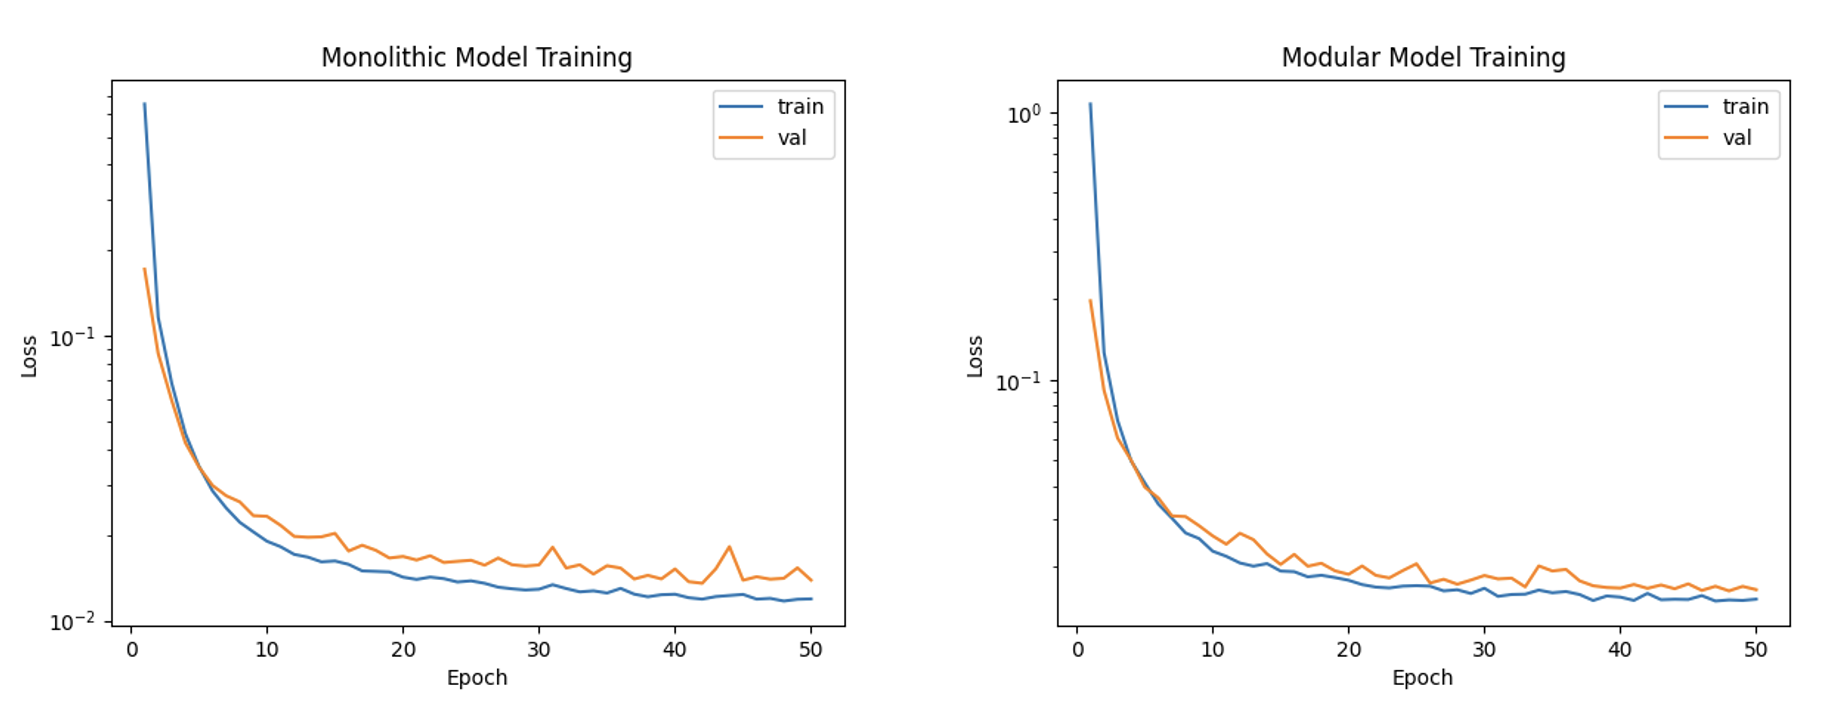
\includegraphics[width=0.8\linewidth]{figs/train_curves_ABC.png}
    \caption{Training curves for the three-node chain. Left: monolithic model.
    Right: modular model. Both converge rapidly and stably.}
    \label{fig:3node_train}
\end{figure}

\subsubsection{Zero-shot performance under intervention}
Without retraining, performance degrades severely for both architectures:
\[
\begin{aligned}
\text{Monolithic:} &\quad \mathrm{MSE_{base}} = 0.0138,\qquad
                           \mathrm{MSE_{interv}} = 4.8165, \\
\text{Modular:}    &\quad \mathrm{MSE_{base}} = 0.0125,\qquad
                           \mathrm{MSE_{interv}} = 4.8015.
\end{aligned}
\]
Figure~\ref{fig:zero-shot} shows that the two architectures are essentially
indistinguishable under zero-shot evaluation: architectural decomposition alone
does not confer robustness when the functional form of a mechanism changes severely.

\begin{figure}[H]
    \centering
    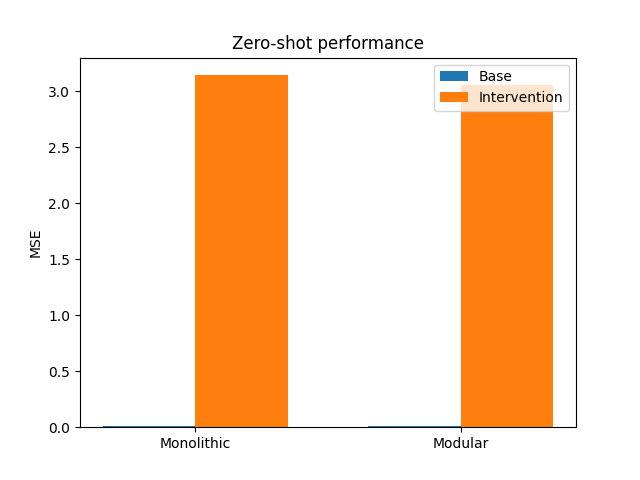
\includegraphics[width=0.45\linewidth]{figs/zero_shot_bar_ABC.png}
    \caption{Zero-shot MSE for both architectures under the upstream intervention
    (three-node chain). Neither model generalizes across the severe functional shift.}
    \label{fig:zero-shot}
\end{figure}

\subsubsection{Few-shot adaptation}
Given $1{,}000$ interventional samples, both models adapt quickly from an initial
MSE near $4.80$ (Figure~\ref{fig:few-shot}):
\[
\begin{aligned}
\text{At 100 steps:}\quad
    &\mathrm{MSE_{mono}} = 0.5800,\qquad \mathrm{MSE_{mod}} = 0.6750, \\
\text{At 1000 steps:}\quad
    &\mathrm{MSE_{mono}} = 0.1303,\qquad \mathrm{MSE_{mod}} = 0.1561.
\end{aligned}
\]
The monolithic model adapts slightly faster in early steps, while the modular model
reaches comparable final accuracy while updating substantially fewer parameters.
This demonstrates the core practical advantage of modular design: parameter-efficient
adaptation to localized mechanism changes.

\begin{figure}[H]
    \centering
    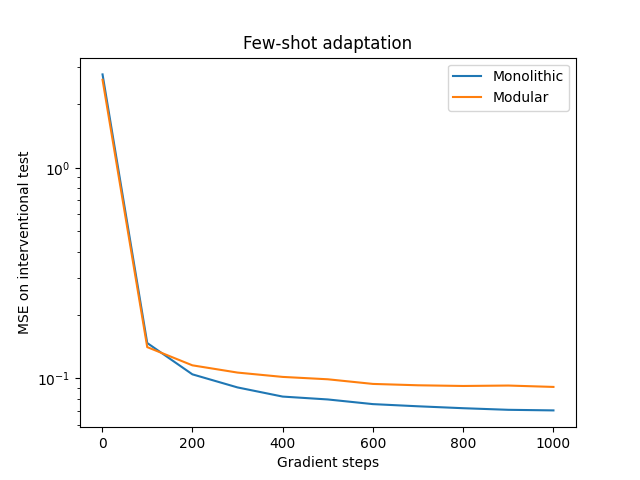
\includegraphics[width=0.45\linewidth]{figs/few_shot_curves_ABC.png}
    \caption{Few-shot adaptation curves (three-node chain, $n=1000$). The modular
    model updates only $f_{AB}$; the monolithic model updates all parameters.}
    \label{fig:few-shot}
\end{figure}

\subsubsection{Adaptation efficiency across sample sizes}
To characterize how the modular advantage scales with available supervision, we
vary the number of interventional samples ($n \in \{50, 100, 200, 400, 500\}$).
Full adaptation curves appear in Appendix~\ref{appendix:three-node-fewshot}.
The modular architecture shows the greatest relative advantage in the low-data
regime: with $n=50$, it achieves MSE $0.343$ versus $0.450$ for the monolithic
model (a 24\% relative improvement). This advantage persists at $n=100$
(0.223 vs.\ 0.258; 14\%) and $n=200$ (0.144 vs.\ 0.171; 16\%), and narrows at
$n \geq 400$, where both models converge to similar performance. The pattern
indicates that the benefit of localizing updates to the perturbed module is
greatest precisely when interventional data are scarce.

\subsection{Four-Node Chain ($A \rightarrow B \rightarrow C \rightarrow D$)}
\label{sec:four-node-results}

\subsubsection{In-distribution performance}
Both models learn the four-node process successfully. The monolithic model achieves
MSE $0.0314$; the modular model achieves $0.0281$. The performance gap is larger
than in the three-node case, consistent with the hypothesis that deeper causal
chains provide more intermediate structure for modular models to exploit.

\subsubsection{Zero-shot performance under intervention}
Under the same upstream intervention, both models degrade substantially:
$\mathrm{MSE_{mono}^{interv}} = 3.5171$ and
$\mathrm{MSE_{mod}^{interv}} = 3.4160$.
As in the three-node case, neither architecture generalizes zero-shot. The modular
model's slightly smaller degradation suggests that causal depth may amplify the
benefit of structural alignment (Appendix~\ref{appendix:four-node}).

\subsubsection{Few-shot adaptation}
With $1{,}000$ interventional samples and updating only $f_{AB}$ for the modular
model, both architectures recover strong predictive accuracy:
$\mathrm{MSE_{mono}^{fewshot}} = 0.0952$ and
$\mathrm{MSE_{mod}^{fewshot}} = 0.0838$.
Unlike the three-node setting-where the monolithic model was faster early on-the
modular model here achieves better final accuracy despite updating far fewer
parameters. Greater causal depth therefore strengthens both the accuracy and
parameter-efficiency advantages of localized modular adaptation
(Appendix~\ref{appendix:four-node}).


\section{Discussion}
\label{sec:discussion}

Our results establish two empirical regularities. First, in-distribution
performance does not differentiate the architectures: modular decomposition is
neither a handicap nor a meaningful advantage when the generative process is
stationary. Second, when a single upstream mechanism changes, modular models adapt
more efficiently, with advantages that grow at lower data volumes and greater causal
depths.


Even though the modular model's sub-networks directly correspond to the generative
mechanisms, the upstream module has learned a specific functional form that is
invalidated by the intervention. Robustness to such shifts would require either
uncertainty-aware modules capable of detecting mechanism change, or a prior over
functional families broad enough to accommodate the shift without retraining.

Several limitations constrain the generalizability of these findings. The causal
chain is low-dimensional and the mechanisms are hand-designed; it is unclear whether
the observed patterns hold in higher-dimensional settings with overlapping or
partially observed causal factors. The modular model also requires clean
separability of mechanisms and local supervision for each module-assumptions that
rarely hold without domain knowledge. Extending these comparisons to settings where
modular boundaries must be discovered from data, and to applied domains such as
healthcare or robotics where mechanisms are known to shift over time, are natural
next steps.


\section{Conclusion}
\label{sec:conclusion}

We compared modular and monolithic neural architectures in controlled causal-chain
environments, isolating the contribution of structural alignment with the generative
process. Modular models match monolithic models in-distribution while offering
clear parameter-efficiency advantages under few-shot adaptation to a localized
mechanism change-with the largest gains in low-data regimes and deeper causal
chains. Neither architecture achieves zero-shot robustness under severe functional
shifts, pointing to the need for richer modular designs that incorporate
mechanism-change detection or broader functional priors.


% 
% Required sections for Neural Networks / Elsevier submission
%


% \section*{Declaration of generative AI use}
% If AI tools were used during preparation, complete this section. Example:
% "During the preparation of this work the author used [TOOL] in order to [REASON].
% After using this tool, the author reviewed and edited the content as needed and
% takes full responsibility for the content of the published article."
% If no AI tools were used, this section may be omitted.

\newpage

\bibliographystyle{apalike}
\bibliography{references}


\appendix
\section{Additional Experimental Results}
\label{appendix:additional-results}

\subsection{Few-Shot Adaptation Across Sample Sizes (Three-Node Chain)}
\label{appendix:three-node-fewshot}

Figure~\ref{fig:appendix-three-node-fewshot} shows adaptation curves for
$n \in \{50, 100, 200, 400, 500\}$ interventional samples in the three-node chain.
The modular model updates only $f_{AB}$; the monolithic model fine-tunes all
parameters. Across all sample sizes the modular model achieves comparable or lower
final error while using substantially fewer parameters, with the advantage most
pronounced at small $n$.

\begin{figure}[htbp]
    \centering
    \begin{subfigure}{0.45\textwidth}
        \centering
        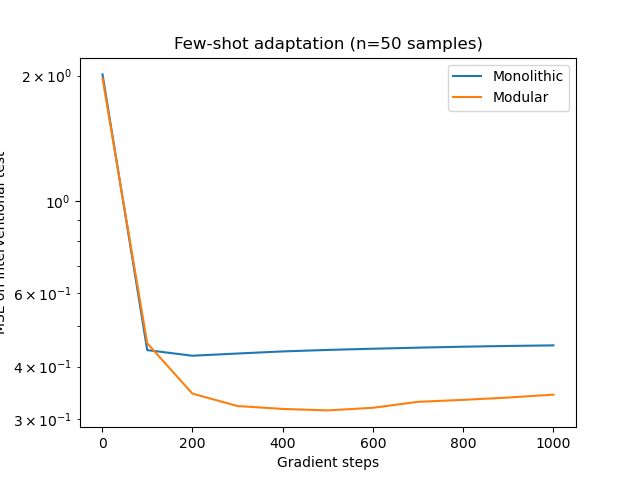
\includegraphics[width=\linewidth]{figs/few shot experiments/n=50.png}
        \caption{$n=50$}
    \end{subfigure}
    \hfill
    \begin{subfigure}{0.45\textwidth}
        \centering
        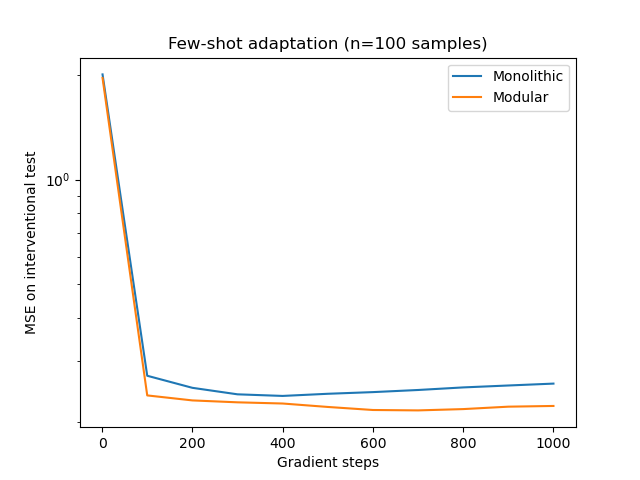
\includegraphics[width=\linewidth]{figs/few shot experiments/n=100.png}
        \caption{$n=100$}
    \end{subfigure}
    \vspace{0.6em}
    \begin{subfigure}{0.45\textwidth}
        \centering
        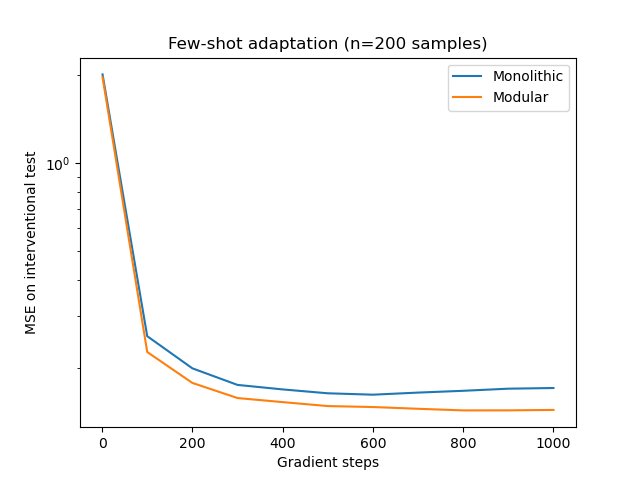
\includegraphics[width=\linewidth]{figs/few shot experiments/n=200.png}
        \caption{$n=200$}
    \end{subfigure}
    \hfill
    \begin{subfigure}{0.45\textwidth}
        \centering
        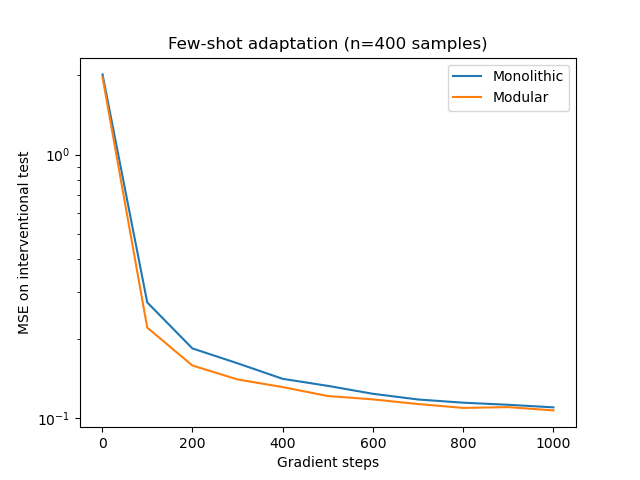
\includegraphics[width=\linewidth]{figs/few shot experiments/n=400.png}
        \caption{$n=400$}
    \end{subfigure}
    \vspace{0.6em}
    \begin{subfigure}{0.45\textwidth}
        \centering
        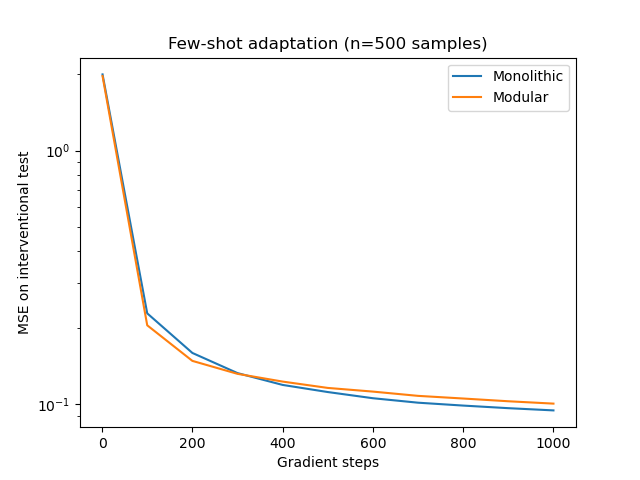
\includegraphics[width=\linewidth]{figs/few shot experiments/n=500.png}
        \caption{$n=500$}
    \end{subfigure}
    \caption{Few-shot adaptation behavior in the three-node chain across varying
    interventional sample sizes.}
    \label{fig:appendix-three-node-fewshot}
\end{figure}

\subsection{Full Results for the Four-Node Chain}
\label{appendix:four-node}

\begin{figure}[htbp]
    \centering
    \begin{subfigure}{0.45\textwidth}
        \centering
        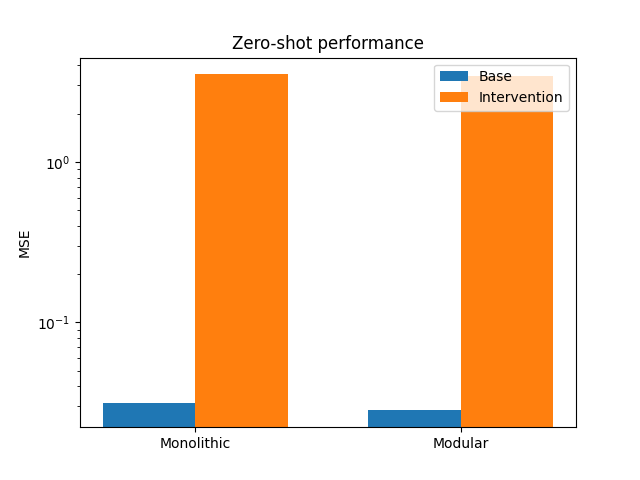
\includegraphics[width=\linewidth]{figs/zero_shot_bar_ABCD.png}
        \caption{Zero-shot performance under intervention.}
        \label{fig:appendix-zero-shot-four}
    \end{subfigure}
    \hfill
    \begin{subfigure}{0.45\textwidth}
        \centering
        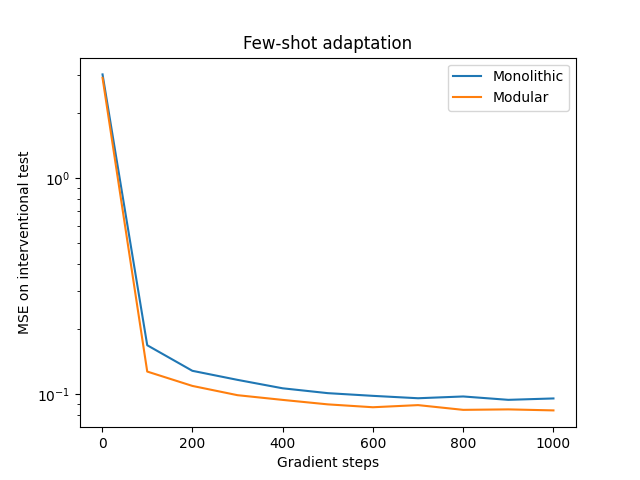
\includegraphics[width=\linewidth]{figs/few_shot_curves_ABCD.png}
        \caption{Few-shot adaptation ($n=1000$).}
        \label{fig:appendix-few-shot-four}
    \end{subfigure}
    \caption{Evaluation results for the four-node chain. Left: zero-shot
    generalization under the upstream intervention. Right: few-shot adaptation.}
    \label{fig:appendix-four-node-eval}
\end{figure}

\begin{figure}[H]
    \centering
    \begin{subfigure}{0.45\textwidth}
        \centering
        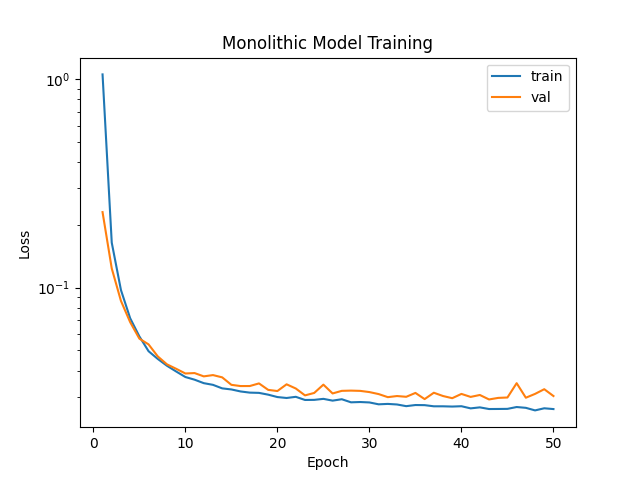
\includegraphics[width=\linewidth]{figs/train_curves_ABCD_mono.png}
        \caption{Monolithic model.}
        \label{fig:appendix-mono-train-four}
    \end{subfigure}
    \hfill
    \begin{subfigure}{0.45\textwidth}
        \centering
        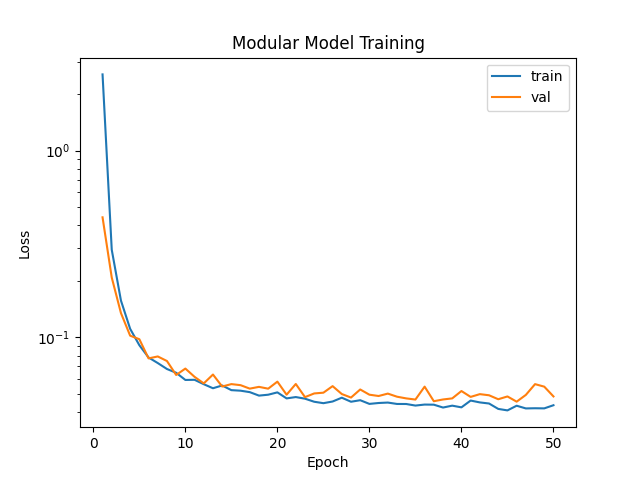
\includegraphics[width=\linewidth]{figs/train_curves_ABCD_mod.png}
        \caption{Modular model.}
        \label{fig:appendix-mod-train-four}
    \end{subfigure}
    \caption{Training curves for the four-node chain. Both models converge stably,
    with the modular architecture achieving slightly lower final error.}
    \label{fig:appendix-four-node-train}
\end{figure}

\end{document}